\chapter{Architektur}

\section{Übersicht}

Um die beschriebenen Funktionalen- und Nicht-Funktionalen Anforderungen erfüllen zu können, haben wir die folgende Architektur entwickelt. \\
Um eine Drohne über einen Server in der Cloud steuern zu können, muss diese mit dem Internet verbunden werden. Um dies zu erreichen verwenden wir ein Smartphone, dass auf der Drohne angebracht wird und über USB mit dem Flight-Controller verbunden ist.  (siehe Abb. \ref{fig:architecture-overview}). Das Smartphone wird aber auch benötigt um dem Drone-Operator ein Benutzeroberfläche zur Verfügung zu stellen, die das Beladen und das Abfragen des Zustands der Drohne ermöglichen. \\
%
\begin{figure}[h]
	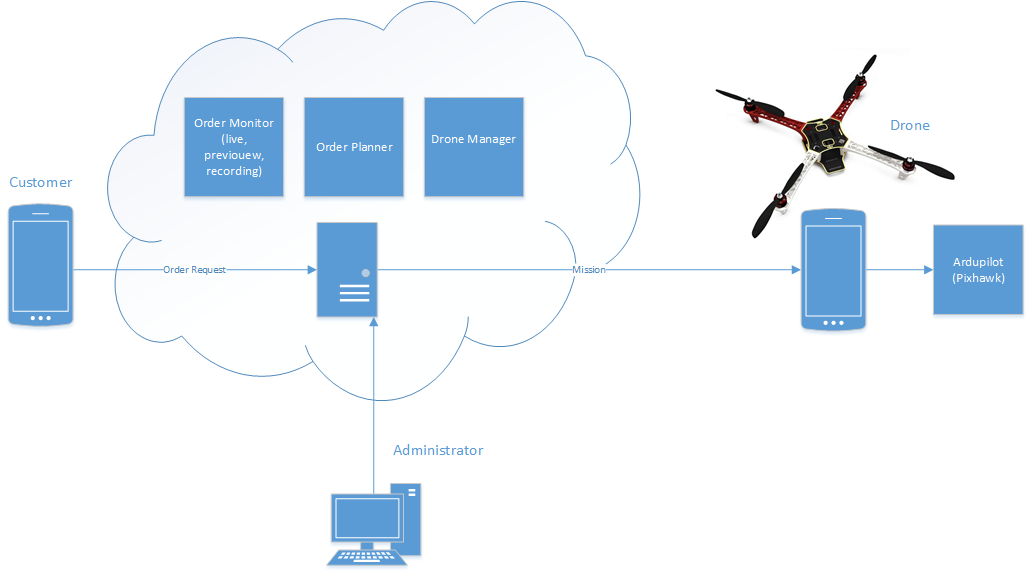
\includegraphics[width=1.0\textwidth]{images/Overview-Diagram.png}
	\caption{Übersicht der Project Helin Architektur }
	\label{fig:architecture-overview}
\end{figure}
%
\section{Kommunikations-Architektur}
Die Abbildung \ref{fig:communication-architecture-overview} zeigt die Kommunikations-Architektur in der Übersicht. Wichtig sind vor allem die verschiedenen verwendeten Protokolle, die benötigt werden um die Anforderungen erfüllen zu können. Bei den mobilen Geräten wird Messaging ({\Gls{AMQP}) verwendet, um bidirektionale Kommunikation zu ermöglichen. Dies ist nötig, damit Kunden und Administratoren die Bewegungen der Drohne live verfolgen können. Die eingesetzte Technologie für die Kommunikation zwischen dem Server und den Smartphones muss ausserdem den Nicht-Funktionalen-Anforderungen gerecht werden im Bezug auf Verbindungsabbrüche und Verbindungswiederherstellung.
%
\begin{figure}[h]
	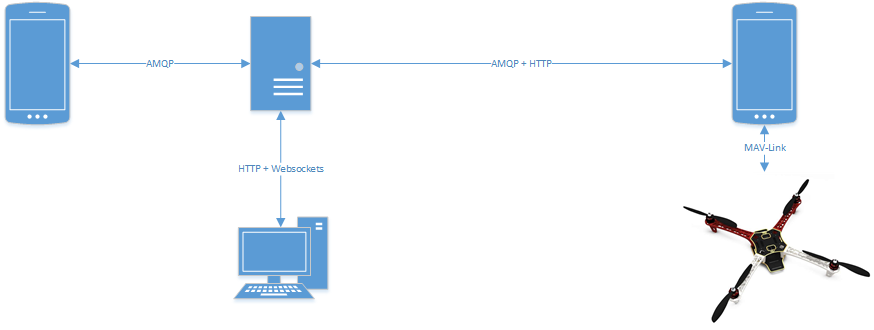
\includegraphics[width=1.0\textwidth]{images/Communication-Overview-Diagram.png}
	\caption{Übersicht der Kommunikations-Architektur mit den jeweiligen Protokollen. }
	\label{fig:communication-architecture-overview}
\end{figure}
%
\subsection{Verwendete Enterprise Integration Patterns}
Messaging-Systeme und Protokolle bieten meistens eine grosse Auswahl an Patterns die verwendet werden können. Für dieses Projekt benötigen wir nur einen kleinen Teil davon um den gestellten Anforderungen gerecht zu werden.
%
\subsubsection{Point-to-Point Channel}
Um zwischen einer registrierten Drohne und dem Server einen sicheren und zuverlässigen Nachrichtenaustausch zu ermöglichen, wird jede Drohne bzw. jede App über einen separaten Point-to-Point Channel angebunden. Der Channel wird nach der Registrierung zugeteilt und stellt den Point-to-Point Kanal zwischen Drone und Server dar. Dies garantiert dem Server eine Nachricht an garantiert eine Drohne zu schicken.
%
\subsubsection{At-most-once delivery}
% Why not exactly once?!
Wir müssen sicher sein, dass eine Drohne eine Mission oder einen Befehl nur ein Mal erhält. Ansonsten müsste Logik eingebaut werden, die diese Problematik löst. Sollte die Drohne einen Befehl oder eine Mission gar nicht erhalten, weil die Verbindung unterbrochen ist, muss das System dies wissen und entsprechend reagieren können.
%
\subsubsection{Event-driven Consumer}
Alle Aktoren des Systems müssen die Möglichkeit bieten auf Grund von Events bzw. Nachrichten Aktionen auszuführen. Beispielsweise:
%
\begin{itemize}
	\item Drohne erhält neue Mission vom Server und soll dies dem Drone-Operator anzeigen.
	\item Server erhält neue Position von der Drohne und soll diese Nachricht dem Kunden weiterleiten und dem Administrator auf dem Web-Client anzeigen.
	\item Smartphone des Kunden erhält neue Position der Drohne, auf der Karte wird die Position der Drohne angezeigt.
\end{itemize}

\subsection{Messages}
Um die Messages sowohl auf dem Server als auf den Android Apps nutzen zu können, müssen alle Messages zu jeder Zeit überall verfügbar sein. Daher wurde ein seperates Projekt angelegt. Es wird jeweils nach MavenLocal deployed um es in den anderen Projekten verfügbar zu machen.
\subsection{Register Drone}
%
\begin{figure}[h]
	\centering
	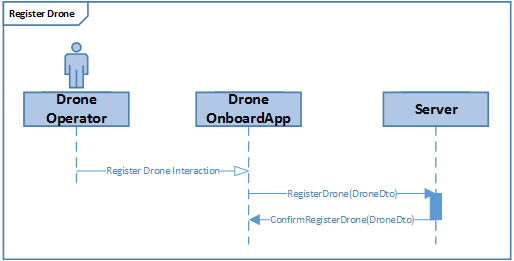
\includegraphics[scale=1.0]{images/registerDrone.png}
	\caption{Übersicht der Project Helin Architektur }
	\label{fig:registerDrone}
\end{figure}
%
\subsection{Order Cargo}
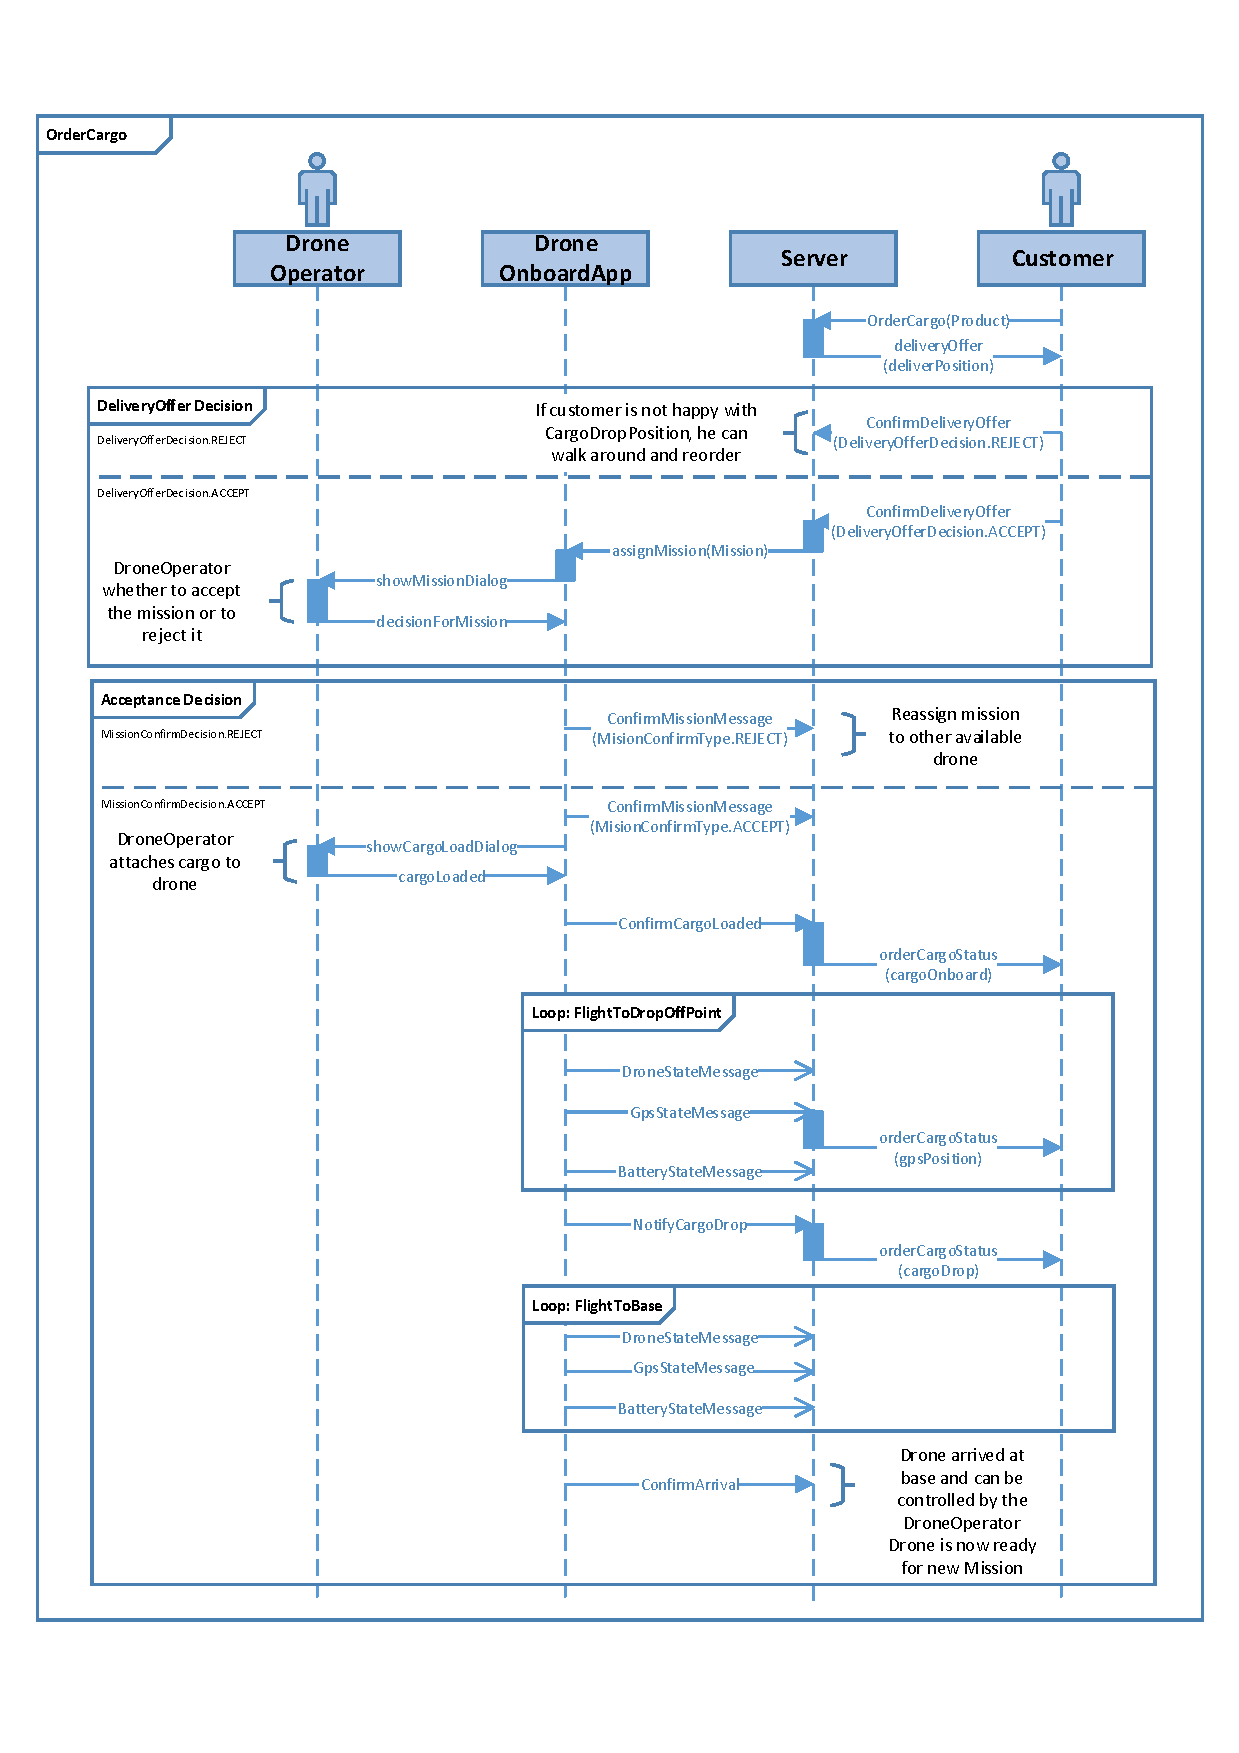
\includepdf[pages=-]{images/OrderCargo.pdf}
Order Cargo beschreibt den Bestellprozess und die damit zusammenhängende Kommunikation. \\
Der User möchte gerne an einem Anlass ein Produkt bestellen. Er bestellt mittels der App ein Produkt, der Server bestätigt ihm die Bestellung und schlägt einen Abwurfort vor. Sollte der Abwurfort dem Kunden nicht entsprechen, so kann er den Prozess abbrechen und ihn nocheinmal auslösen, sobald er sich in einer geografisch glücklicheren Lage befindet.
\\
Der Server evaluiert im Anschluss welche Drone den Auftrag ausführen kann gerade verfügbar ist und schlägt die Mission dem DroneOperator vor. Sollte die Drone verfügbar sein, so kann er diesen Auftrag bestätigen. Im Fall einer Wartungsarbeit kann der Auftrag zu diesem Zeitpunkt auch abgelehnt werden. Sobald der Auftrag angeommen wurde erhält der DroneOperator genaue Angaben zur Beladung der Drohne. Anschliessend wird die Ladung bestätigt und der Server kann dem Kunden mitteilen, dass die Drone nun startklar ist. Während des Fluges erhält der Kunde Benachrichtigungen vom Server mit der aktuellen Position der Drohne. Sobald die Ladung abwurfbereit ist, wird der Kunde informiert und die Drohne kann die Ladung abwerfen. Im Anschluss fliegt die Drohen zur Basis zurück und bestätigt dem Server die Ankunft, so kann gewährleistet werden, dass die Drohne wieder eine eine Mission erhalten kann.
%